\documentclass{article}
\usepackage{graphicx}
\usepackage{amsmath}
\usepackage{natbib}
\usepackage{xcolor}
\usepackage{amssymb}

\usepackage{algorithm}
\usepackage{algpseudocode}

\usepackage{rotating}
\usepackage{tikz}


\newtheorem{proof}{Proof}
\newtheorem{lemma}{Lemma}
\usepackage[margin=1in]{geometry}

\begin{document}


\title{Sequential Cognition Processes: A Framework For Reasoning with Non-Monotonic Logics}
\author{Axel Ind \\ axeltind@gmail.com \\ University of Freiburg}

\maketitle

Research Question: \textit{``Is there a way to systematically represent some (or all) non-monotonic logics in a framework that standardises cognitive modelling under these logics without sacrificing their expressiveness?"}

\section{Overview}
For my Master's thesis I intend to describe, implement, and test a novel framework for modelling human reasoners called the Sequential Cognitive Process. SCPs retain most of the expressiveness of the hitherto \textit{ad hoc} approaches to modelling reasoners with non-monotonic logics, but also introduce a number of desirable properties:
\begin{enumerate}
\item They enable modelling of individual reasoners through addition or subtraction of well-described mental operations. This is in contrast to most non-monotonic logic approaches which can model the general reasoner across a number of cognitive tasks but do not extend well to explaining reasoning that deviates from the norm.
\item They standardise a broad class of non-monotonic logical frameworks so that cognitive comparisons, even across different frameworks are possible, in particular I have given some thought to the use of string-matching algorithms borrowed from the field of bioinformatics (such an extended version of the Needleman Wunsch Aglorithm\cite{needleman1970general}) to comparing WSTs as operation sequences.
\item Because they are sequential (essentially linked lists of mental operations) they lend themselves well to traditional search techniques, and their utility in finding -- though not yet justifying -- models of the Suppression Task has already been demonstrated for both general and individual reasoners.
\item They standardise a set of well-founded cognitive processes (such as, the Suppression Effect, Affirmation of the Antecedent, Conjunction Fallacy bias, and the introduction of abnormalities) as reusable epistemic operations which can be constrained or expanded according the needs of the researcher.
\item Because they are sequential sequences of actions, there is certainly potential for traditional heuristic approaches to problem solving.
\end{enumerate}

An existing implementation of this system has already been implemented\footnote{Available on Github: https://github.com/AxelInd/SequentialCognitionPrcoesses. For access, please contact me with your details.} with a focus on the Weak Completion Semantics \citep{holldobler2015weak}. This implementation has proved effective at modelling both the \citep{byrne1989suppressing} and the Wason Selection Task \citep{wason1968reasoning}, with work to expand the implementation ongoing.

\section{What is an SCP}

An SCP is a model of a reasoner, whether individuals or a group. The SCP assumes that some epistemic state (of whatever form the nonmonotonic logic requires) is modified by mental operations in the SCP to reach a final epistemic state that satisfies some goal properties. An SCP Problem $\pi=(s_i,\gamma,M)$ describes the requirements and limitation of the SCP before it is created\footnote{This formulation is inspired by the field of AI Planning}. $s_i$ contains the initial state of the SCP, and $\gamma$ is the goal of the SCP (e.g. to mimic the classical case of the Suppression Task), $M$ is the set of allowable cognitive operations.

The SCP framework makes several core assumptions about the nature of cognition:


\begin{enumerate}
\item Evolving Epistemic States: SCPs are built on the idea that some mental model of the world exists before the problem-solving begins (even if the model is empty), and is updated by each mental process that acts on it, yielding a new epistemic state as output from mental process $m_n$ to be used as input for mental process $m_{n-1}$.
\item Sequential Reasoning: the assumption that a reasoner will perform only one mental operation at a time before moving on to the next one. Although it initially seems very limitting, the complexity of mental operations is unconstrained, and could itself involve parallel processes provided that a unified mental state is achieved before the next operation begins.
\item Reusable Operations: in order to be more than just a container for some other non-monotonic logic, cognitive tasks must share at least some complex operations. If this were not the case, standardising a set of cognitive operations to model unseen tasks would be impossible. Fortunately, there is ample evidence of consistent mental approaches to reasoning \citep{ragni2017formal}.
\item Limited mental processing power: SCPs assume a sequential and finite number of mental operations to reach a goal. Without this property, it would be impossible to accurately model human cognition. Further, there would be no reasonable scoring system for determining the best explanation when multiple SCPs all model the same thought process (the simplest scoring system intuitively simply being the length of the two SCPs and preferring the smaller).
\end{enumerate}



\section{State of the Art}

\subsection{More Questions Than Answers}
The example of the Suppression Task @TODORef illustrates one of the glaring problems with cognitive modelling in non-monotonic reasoning as it stands at present: it is unstructured. What rules should be followed when adding abnormalities? How do we choose the order to apply these operations? Is this the only reasonable sequence in which to apply these operations? All these questions arise from a lack of structure in the frameworks being used. For example, work by @TODORef discusses the idea of obligate and factual conditionals, which are treated differently in terms of how abnormalities are added. From this it immediately follows that extensions to the WCS are possible, but where can they occur? Which extensions and changes are well founded in the psychological literature? What are the properties of the search spaces of these extensions? Is it even possible to compare different cognitive models to one other if they produce identical output? SCPs are an attempt to create a framework for non-monotonic logics that is suitable to answer these questions.

One of the most important questions to answer, is if it possible for these non-monotonic logics to model individual reasoners as well as general reasoners. Work by @TODOref showed that simple extensions to the Weak Completion Semantics allowed researchers to model the four most common decisions of participants in the Wason Selection Task. There is significant potential for research into modelling the unusual choices of participants who do not conform to the normally observed results. Part of my thesis will be dedicated to justifying a view of these unusual reasoners as deviations from the normal cognitive process who still follow a very similar reasoning approach but with small and well-founded differences when compared to general reasoners. In @TODO we briefly discuss this idea in terms of the Suppression Task.

\subsection{Example: The Suppression Task}
\subsubsection{What is the Suppression Task?}
The Suppression Task refers to an experiment conducted by @TODO in @TODO and is classical example of the inadequacy of monotonic logics for modelling human reasoning. In classical logic, if our knowledge base $kb$ is such that $kb \models \phi$, then it must be the case that $kb \cup \psi \models \phi$. However, in the suppression task participants no longer draw classically valid inferences when new information is added. The task is often formulated as follows:

\begin{itemize}
\item $e \rightarrow l$: If she has an essay to write ($e$), she will study late in the library ($l$).
\item $\top \rightarrow e$: She has an essay to write ($e$).
\item $o\rightarrow l$: If the library is open ($o$), she will study late in the library ($l$).
\end{itemize}

Given only the rules $(e \rightarrow l)$ and $(\top \rightarrow e)$, the participants consistently concluded that she would study late in the library, seemingly drawing the classical logic inference $\frac{e \rightarrow l, e}{l}$ with \textit{modus ponens}. But when given the additional rule $o\rightarrow l$, participants no longer believe that they have enough information to judge whether she will study late in the library, and a significant portion of them no longer draw the classical conclusion. This effect, called Suppression, demonstrates the need for something more than classical logic for modelling human reasoning.

\subsubsection{Modelling the Suppression Task with the WCS}
Work by @TODOref has shown that the Weak Completion Semantics is an adequate non-monotonic logic for modelling the Suppression Task. The reader is assumed to be familiar with the Weak Completion Semantics and so it is only briefly discussed here.

Under the Weak Completion Semantics and \L ukasiewicz 3-valued logic the task is usually modelled as follows for the case without suppression:
\begin{enumerate}
\item Initial logic program: $P = \{e \rightarrow l, \top \rightarrow e \}$. This program represents the task without information about what happens if the library is open.
\item Addition of Abnormality: $P = \{e \land \lnot ab_1 \rightarrow l, \top \rightarrow e, \bot \rightarrow ab_1 \}$. The program now reflects the possibility that some abnormal event may prevent her from going to the library, but because we have no information about the nature of this event, it is set to false by default.
\item Weak Completion: $wc(P) = \{e \land \lnot ab_1 \leftrightarrow l, \top \leftrightarrow e, \bot \leftrightarrow ab_1 \}$. Weak completion @TODOappendixref is applied to the logic program and, in this case, only implications need to be changed to bijections.
\item Semantic Operator:
\begin{itemize}
\item $\top=\{e\}, \bot=\{ab_1\}$
\item $\top=\{e,l\}, \bot=\{ab_1\}$
\end{itemize}
\end{enumerate}

After application of the semantic operator $l$ is true in the least model, and so participants conclude that she will study late in the library (as when $P$ is evaluated classically). However, in the case where Suppression is observed, the same process yields a different result because of the presence of the extra conditional ($o\rightarrow$).
\begin{enumerate}
\item Initial logic program: $P = \{e \rightarrow l, \top \rightarrow e, o \rightarrow l \}$. The initial program now includes information about the extra (suppressing) conditional.
\item Addition of Abnormality: $P = \{e \land \lnot ab_1 \rightarrow l, o \land \lnot ab_2 \rightarrow l, \top \rightarrow e, \lnot o \rightarrow ab_1, \lnot e \rightarrow ab_2 \}$. Adding abnormalities is a poorly described process and often relies on intuitionist views of what actually constitutes an abnormal situation. In this case we adopt the practise of identifying abnormalities as described in Appendix~\ref{ssec: addAbnormalities}.
\item Weak Completion: $wc(P) = \{((e \land \lnot ab_1) \lor (o \land \lnot ab_2)) \leftrightarrow l, \top \leftrightarrow e, \lnot o \leftrightarrow ab_1, \lnot e \leftrightarrow ab_2 \}$. Weak completion is applied to the logic program, combining rules with shared heads and replacing implications with bijections.
\item Semantic Operator:
\begin{itemize}
\item Execution 1: $\top=\{e\}, \bot=\{ab_2\}$
\end{itemize}
\end{enumerate}

Now suppression has been displayed in the logic program and the variable $l$ remains unknown in the least model.

\subsubsection{Modelling the Suppression Task with the SCPs}
\begin{figure}
\begin{center}
 \centering 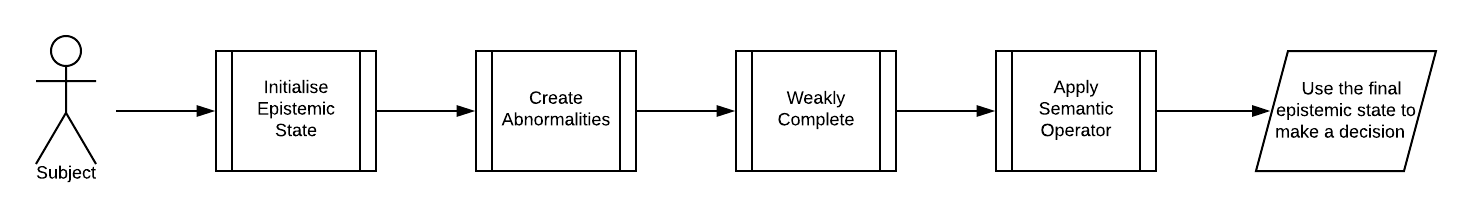
\includegraphics[scale=0.65]{suppressionSCP_overview}
\caption{A generalised illustration of the WCS in an SCP. }
\label {fig:supoverview}
\end{center}
\end{figure}

\begin{figure}
\begin{center}
 \centering 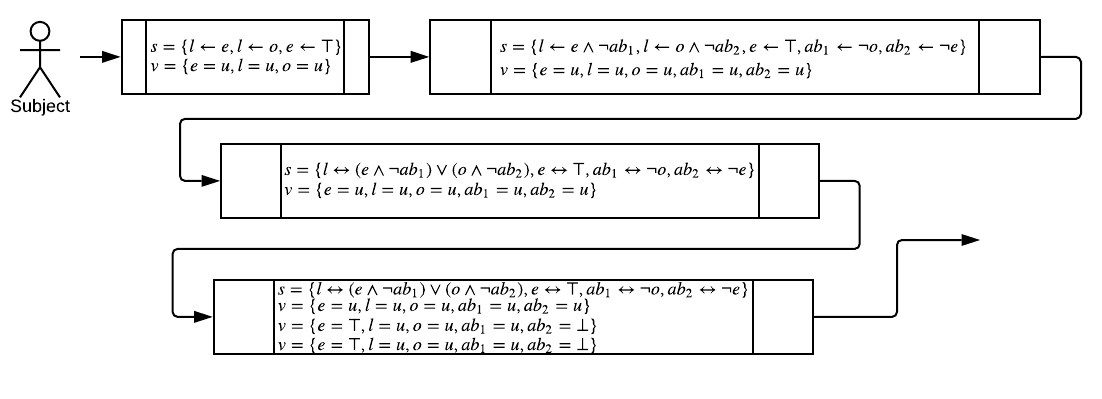
\includegraphics[scale=0.75]{suppressionSCP_normal}
\caption{The standard case of the Suppression Task, demonstrating the suppression effect. Where the epistemic state in the boxes represents the output of that cognitive operation.}
\label {fig:supnormal}
\end{center}
\end{figure}

Figure~\ref{fig:supoverview} illustrates a generalised process to describe the Suppression Task as a series of sequential steps, each process passing information to the next process\footnote{It is important to note that a diagram like this is valid for \textit{any} cognitive modelling task because any process may be arbitrarily complex and non-sequential. and so the overall linear process of (actor, complex decision, observed results) is always valid for retroactive modelling, and at least as powerful as the non-monotonic logic framework it uses for modelling.}

Under SCPs the implicit sequence of operations in the Suppression Task are systematized and refined into complex operations. Every complex operation takes as its input an epistemic state $s_i$ and outputs an epistemic state $s_{i+1}$ to be used as input to the next complex operation. For the Weak Completion Semantics it suffices to add an initial epistemic state $s_i=(KB,V)$ consisting of a set of rules $KB$, and a set of variable assignments $V$ (in the case of the Wason Selection Task additional information about obligate and factual conditions can be added to model \textit{modus tolens} inferences in the WCS, but that will be discussed in more detail in a later paper).

One interpretation of the requirements of the suppression task $\pi=(s_i,\gamma,M)$ using SCPs and the WCS is as follows: 
\begin{itemize}
\item $s_i=\{kb_i, v_i\}$
\item $kb_i=\{e \rightarrow l, \top \rightarrow e, o \rightarrow l\}$
\item $v_i=\{e:u, l:u, o:u\}$
\item $\gamma = l\models \top $ or $l \models \bot$ (that is, l is no longer mapped to unknown in the final epistemic state.)
\item $M=\{init, addAB, WeaklyComplete, Semantic Operator\}$
\end{itemize}

where $init$ is always the first cognitive operation and adds the initial variables and rules to epistemic state; $addAB$ adds abnormalities to the current epistemic state using the procedure described in Algorithm~\ref{alg:addAbnormalities} (but now also adds those abnormalities to the variable list of the epistemic state; $Weakly Complete$ weakly completes the knowledge base of the current epistemic state; and the semantic operator returns an epistemic state that leaves the knowledge base unchanged but updates the variables of that state to return the least model of the epistemic state.

Treating Figure~\ref{fig:supoverview} as an SCP, we observe the sequence of output states seen in Figure~\ref{fig:supnormal}. Note that in the final state $l$ remains unknown and the suppression effect is demonstrated.

\subsubsection{Extending the Suppression Task with the SCPs}
One of the most significant tasks of my thesis will be to find and implement a variety of cognitive operations for which there are evidence in the psychological literature. The selection of allowable complex operations $M$ will have a significant impact on which tasks the SCP is able to handle, and only those for which there is supporting evidence should be added.

The previous example merely showed that SCP are suitable for modelling the suppression task. In this example we consider one of the most powerful characteristics of SCPs, the ability to model unusual results as deviations from general reasoning. A significant portion @TODOpercentage of people still believe that she will study late in the library when presented with the suppression task. Several possible explanations are intuitive, the first and simplest, is the assumption that the reasoner is using classical logic and drawing the classical conclusion. However, what if that is not the case? What if they do reason in exactly the same way as the other reasoners, except for one or two small deviations?

In this example we consider two possible deviations that could explain the classical result of the Suppression Task: variable deletion, and variable fixation. Both of these operations will be discussed in a way that may seem overly prosaic to many readers, but the reason for the examples given is to reinforce how reasonably we might expect these cognitive operations occur in reasoning tasks.

\subsubsection*{Variable Deletion}

Consider the sequence of numbers (1, 44 ,27 ,8 ,0 , -4, 6, 7, 346, 7, 74, 7, 234, -55, 2.4, 18). Now without looking back at the numbers, ask yourself some questions: how many numbers were there? Were any of them prime? How many numbers were repeated? In all probability you are not entirely sure. This simple thought experiment provides support for our first extension, the idea that variables can be ``forgotten", that is, that information that existed in the knowledge base at one point in time might no longer exist at a later timepoint. 

This is not the only imaginable case where a variable might be removed from the knowledge base of the person being modelled. The size of the knowledge base used for cognitive modelling is always implicitly restricted to relevant variables, only those variables whose values might reasonably be expected to affect the final conclusions drawn with regard to the research question. Finding which variables and rules are relevant is, however, non-trivial. For another real-life example, imagine a mystery novel. Three hundred pages of plot descriptions, character actions, and dialogues. In a good murder mystery novel every piece of information that reveals the killer's identity is hidden in the story itself, yet we do not hold every fact and interaction in the book in our epistemic model of the book, so discerning the identity of the killer remains a mystery until the last page. But when the mystery is solved, many details that we internalised while reading (and recall in retrospect) suddenly make the conclusion seem obvious. We have not forgotten this information, we had merely incorrectly deemed it irrelevant at the time and ignored it in our cognitive processing.

The exact details of how to delete a variable from a knowledge base is non-trivial, and there is no best practice for doing so. But in simple cases the process can be intuitive. Given $kb={a\leftarrow\top, b\leftarrow \top}$ deleting variable $a$ might be as simple as removing all rules that mention it from the knowledge base (though an argument could also be made that it should be set to unknown).

In the case of the Suppression Task we argue that one cognitively valid reason for drawing the classical conclusion to the task may be forgetting (or disregarding) the variable $o$. Figure~\ref{fig:supmod} illustrates this case, and shows how the insertion of a complex operation can completely change the final epistemic state.

\begin{figure}
\begin{center}
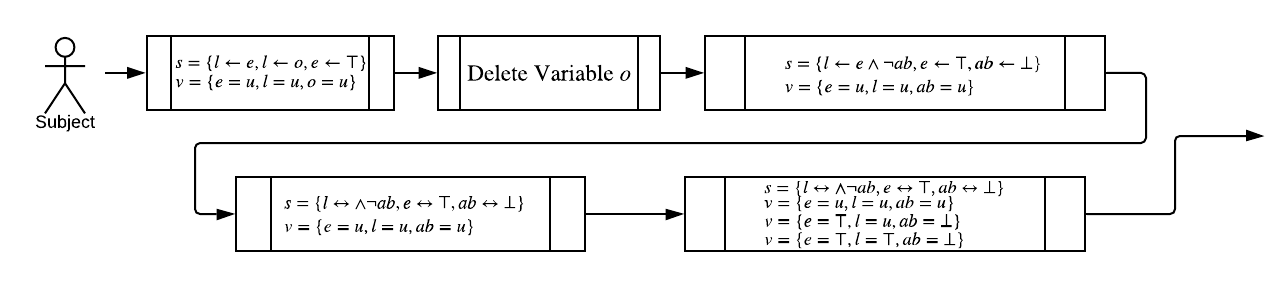
\includegraphics[scale=0.7]{suppressionSCP_mod}
\end{center}

\caption{The Suppression Task in which the additional operation of deleting the variable $o$ occurs.}
\label{fig:supmod}
\end{figure}

\subsubsection*{Variable Fixing}

\begin{figure}
\begin{center}
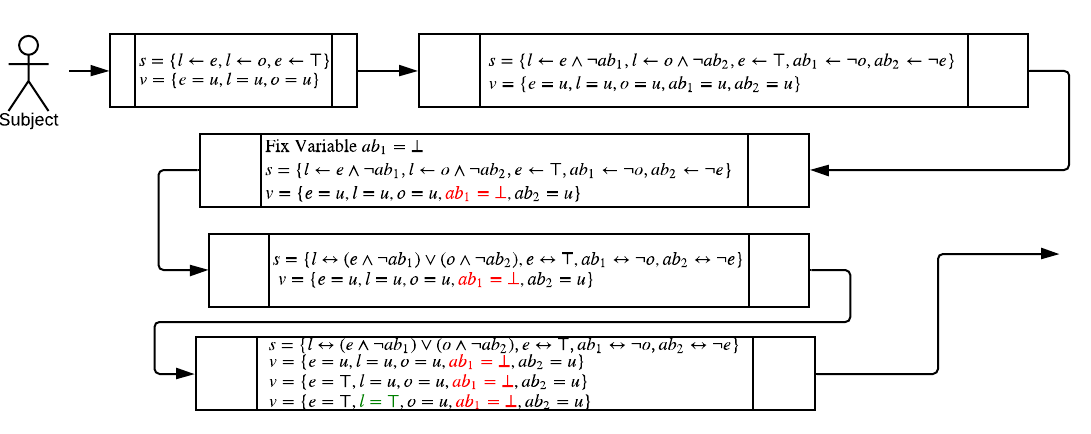
\includegraphics[scale=0.7]{suppressionSCP_mod2}
\end{center}

\caption{The Suppression Task in which the additional operation of fixing the variable $ab_1$ to false occurs.}
\label{fig:supmod2}
\end{figure}

The second case of a potential complex operation to add to the search space of our SCPs is the idea of Variable Fixing. The idea that some  conclusions can be fixed \textit{a priori}. Consider a person who strongly doubts the effectiveness of vaccines, we will call her Karen. Karen started her day convinced that giving her child the MMR vaccine is more dangerous than the disease itself. Later that day Karen spoke to her doctor who strongly advised that she vaccinate her child. He offered her a variety of peer-reviewed papers and studies that showed the relative safety of the vaccination. Karen listened carefully to the trained medical professional, and then went home. After some thought Karen decided that he was wrong, and her opinion on vaccines didn't change.

In this example Karen shows a very powerful type of cognitive bias, the unwillingness to change change her opinions, despite powerful evidence to the contrary. This phenomenon has observed across a great many fields of study, from medical psychology \citep{brown2010omission} \citep{wroe2005feeling} to political sciences\citep{tappin2017heart}. In the context of cognitive modelling with logics, it indicates that a mental rules or variables are immutable, regardless of new evidence or valid beliefs that would logically contradict them. Non-monotonic logics, as a class, are already capable of dealing with bias effect, as non-monotonic logics are built on the basis of a preference operation. However, for the case of the Weak Completion Semantics and SCPs, it serves to introduce a complex operation $fixX$ which can fix the value of a rule or variable at every point after it occurs in the SCP.

In practise this necessitates a way of denoting fixed variables so that future operations do not change them, it also strongly suggests the plausibility of some operation $unfixX$ which would allow a variable to be fixed to a new value again after it occurs. For the purposes of the Suppression Task it suffices to show that the $fixX$ operation can change the conclusions of the general reasoner to those of the deviant reasoner.

Figure~\ref{fig:supmod2} shows the effect of adding a complex operation which fixes the value of the abnormality to false in $v$ so that, no matter what rules are present in $kb$ when the semantic operator is applied, $ab_1$ will remain false\footnote{The question of which solution best models deviant reasoners in the suppression task is one of significant interest and I intend to go into some detail about possible scoring algorithms and heuristics for determining the most likely SCP for a cognitive task when multiple candidate SCPs come to the desired conclusions.}.

\section{Implementation}
A simple implementation of the SCP framework has already been implemented for the WCS, it has been shown able to model both the Suppression Task and the Wason Selection Task in terms of both general and deviant reasoning. The overall structure of the SCP implementation is as a pipeline, a linked list of operations each of which relies on input from the previous operation in the list.

\subsection{Class Diagram}

\begin{sidewaysfigure}
    \centering 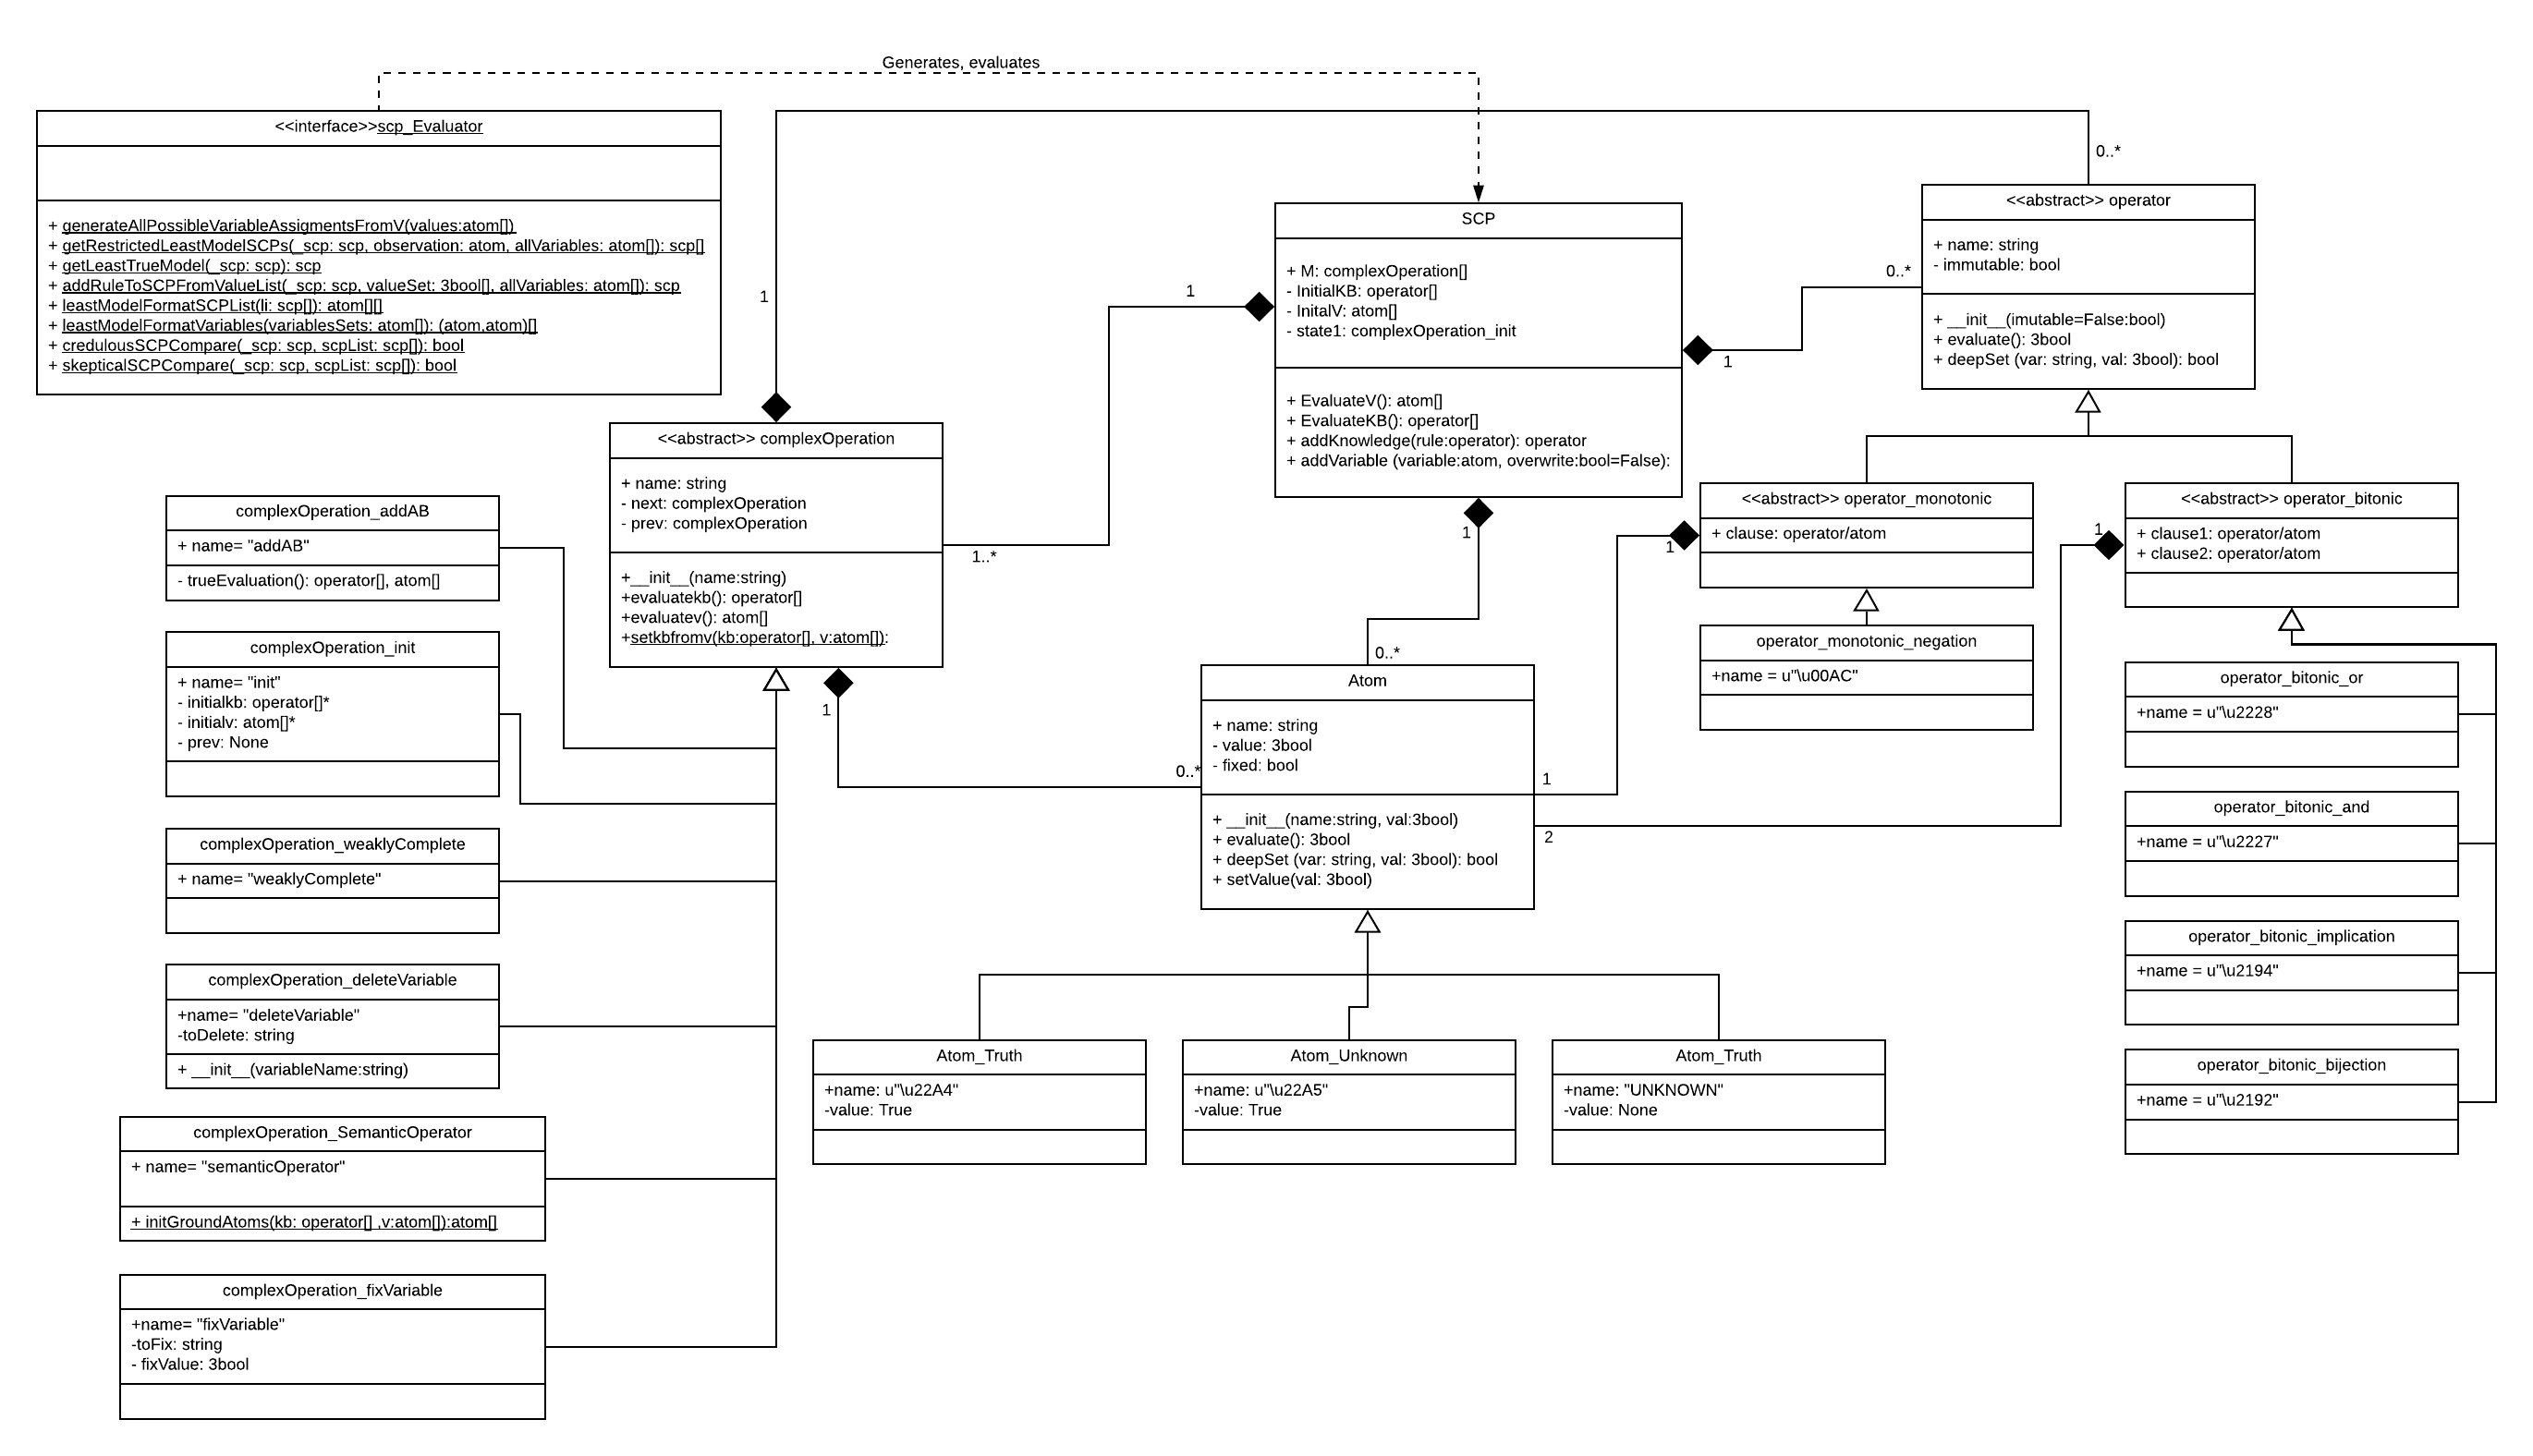
\includegraphics[width=\textwidth]{scpClassDiagram}
    \caption{A simplified illustration of class interactions in the SCP implementation.}
    \label{fig:classDiagram}
\end{sidewaysfigure}

Figure~\ref{fig:classDiagram} shows a simplified class diagram of the implementation of the SCP program. The scp class makes use of a basic implementation of 3-valued logic and a sequence of complexOperation objects in order to evaluate the knowledge base and variables of the SCP after each operation.

Each complexOperation is a pipeline, it contains no data other than pointers to its successor and predecessor and passes the results of its \textit{evaluatev()} and \textit{evaluatekb()} functions to the next operation as input. The code itself is heavily commented and contains filed which implement and execute examples of the Suppression Task and Wason Selection task under WCS.

\subsubsection{Additional Features}
Several other features will be added to the implementation soon:
\begin{itemize}
\item DeNovo Searching: finding an SCP that satisfies a goal condition form scratch, iterating over the set off cognitive operation in $M$. This search is important for coming up with an explanation for the general (most common) results of a cognitive task.
\item Insertion Searching: finding which additional complex operations can be added to an existing SCP to produce results consistent with the deviant reasoner. This search is important for describing unusual results as deviations from the general reasoner. It is also important for scoring the likelihood of these the SCP.
\item Scoring: a modified version of Needleman-Wusch algorithm for string matching has already been theoretically described and must now be implemented in order determine how similar different models are to each other.
\end{itemize}


\section{Milestones}
A portion of the work to create and formalise SCPs has already been completed. A literature review, time spent programming, and time spent formalising the idea of SCPs has already devoted to the problem. however there is still a significant amount of work to be done:
\subsubsection*{Timeline}
\begin{itemize}
\item Standardise implementation interface: 3 Feb - 9 Feb
\item Extend Interface to Conjunction Fallacy under WCS: 10 Feb - 16 Feb
\item Complete paper on SCPs under the WCS: 17 Feb - 23 Feb
\item Conceptually extend SCPs to Reiter's Default Logic: 24 Feb - 1 March
\item Extend the existing implementation to handle Default Logic: 2 March - 8 March
\item Explore scoring algorithms for SCps: 3 March - 9 March
\item Examine application of heuristics to SCPs: 10 March - 15 March
\item Complete paper on SCPs under Default Logic: 16 March - 23 March
\item Write Thesis: 23 March - 20 April
\item Correction, updates, and new ideas: 21 April - ...
\end{itemize}

\subsubsection*{Deliverables}
\begin{itemize}
\item Conference ready paper on SCPs and the WCS: 23 Feb
\item Conference ready paper on SCPs and the default logic: 23 March
\item Complete, documented, extensible implementation of SCPs containing various examples, search functionality, and best-practice design: 1 April
\end{itemize}
	
\bibliography{bibl}
\bibliographystyle{chicago}

\newpage

\section{Appendix}

\subsection{Systematically Adding Abnormalities} \label{ssec: addAbnormalities}
Adding abnormalities is a poorly described process and often relies on intuitionist views of what actually constitutes an abnormal situation. For this reason I have provided one concrete method for adding abnormalities to a logic program (though many others exist and can be extended at will). This particular one is based on the principle that if a variable $v_1$ has the power to make another variable $v_2$ true, then it may be the case that participants believe that any other variables $V'$ satisfying $v_2$ may only do so when $v_1$ holds. This intuition is counter to classical logic, but follows intuitively in cases like the Suppression Task where participants believe that the library not being open may be the reason that the she doesn't study late in the library, even when she has an essay to write. The precise procedure is as follows:


In the case of SCPs, the procedure for creating abnormalities is handled by a single complex epistemic operation and so may be substituted for any competing method with ease without disrupting the flow of the SCP.



\begin{algorithm}
\begin{algorithmic}[1]
\Function{addAbnormalities}{P}
\State \texttt{$P':=[]$}
\For{\texttt{Unique $head$ with $(body \rightarrow head) \in P$}}
\State \texttt{$headDependencies$:= [all non-ground bodies s.t.$(body \rightarrow head) \in P$]}
\For{\texttt{$body_i$ with $(body \rightarrow head) \in P$}}
\State \texttt{$ab_{x}$:=new abnormality} \Comment{Where $x$ is a unique identifier}
\State \texttt{create new rule $head \leftarrow body_i \land \lnot ab_x$} 
\State \texttt {$abDependencies = headDependencies \backslash body_i$}\Comment{$\bot$ if it would be empty}
\State \texttt{$rule$=create new rule $(ab_x \leftarrow dep_1 \land ... \land dep_n)$ for $dep \in abDependencies$}
\State $P'+=rule$
\EndFor
\EndFor
\State \Return $P'$
\EndFunction
\end{algorithmic}
\label{alg:addAbnormalities}
\end{algorithm}




\end{document}
